\section{Establishing De Morgan's Laws of Set Theory}

De Morgan's Laws are rules which are used to relate intersections and unions
through complements. Generally, according to De Morgan's Laws:

\begin{enumerate}
  \item The complement of the union of sets is equal to the intersection of the
  individual complements. This means that if $A$, $B$ and $C$ are sets,
  \[
    (A \cup B)' = A' \cap B', \qquad (A \cup B \cup C)' = A' \cap B' \cap C'.
  \]
  In words: \emph{the complement of the union equals the intersection of the individual complements.}

  \item The complement of the intersection of sets is equal to the union of the
  individual complements. This means that if $A$, $B$ and $C$ are sets,
  \[
    (A \cap B)' = A' \cup B', \qquad (A \cap B \cap C)' = A' \cup B' \cup C'.
  \]
  In words: \emph{the complement of the intersection equals the union of the individual complements.}
\end{enumerate}

Let us use the activity below to validate these rules.

\begin{activity}{Activity 1.1: De Morgan's Laws}
\begin{enumerate}
  \item Make a copy of the diagram below:

  \begin{center}
  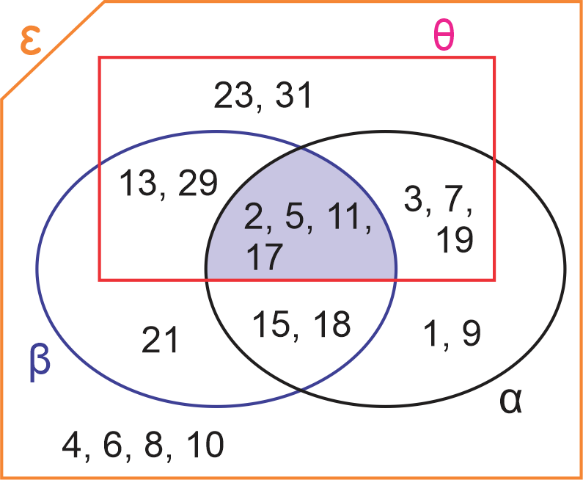
\includegraphics[width=0.7\textwidth]{figures/activity1-1.png}
  \end{center}

  \item List the elements in $\alpha$, $\beta$ and $\theta$.
  \item List the elements in $\alpha'$, $\beta'$ and $\theta'$.
  \item Find (a) $(\alpha \cup \beta \cup \theta)'$ \quad (b) $\alpha' \cap \beta' \cap \theta'$ \quad (c) $(\alpha \cap \beta \cap \theta)'$ \quad (d) $\alpha' \cup \beta' \cup \theta'$.
  \item Compare your result in 4(a) to 4(b). What conclusion can you draw?
  \item Compare your result in 4(c) to 4(d). What conclusion can you draw?
\end{enumerate}
\end{activity}

Compare your answer to the suggested solution below.

\begin{enumerate}[start=2]
  \item
  \begin{align*}
    \alpha &= \{1, 2, 3, 5, 7, 9, 11, 15, 17, 18, 19\}, \\
    \beta &= \{2, 5, 11, 13, 15, 17, 18, 21, 29\}, \\
    \theta &= \{2, 3, 5, 7, 11, 13, 17, 19, 23, 29, 31\}.
  \end{align*}
  \item
  \begin{align*}
    \alpha' &= \{4, 6, 8, 10, 13, 21, 23, 29, 31\}, \\
    \beta' &= \{1, 3, 4, 6, 7, 8, 9, 10, 19, 23, 31\}, \\
    \theta' &= \{1, 4, 6, 8, 9, 10, 15, 18, 21\}.
  \end{align*}
  \item
  \begin{align*}
    \text{(a)}\quad (\alpha \cup \beta \cup \theta)' &= \{4, 6, 8, 10\} \\
    \text{(b)}\quad \alpha' \cap \beta' \cap \theta' &= \{4, 6, 8, 10\} \\
    \text{(c)}\quad (\alpha \cap \beta \cap \theta)' &= \{1, 3, 4, 6, 8, 9, 10, 13, 19, 21, 23, 29, 31\} \\
    \text{(d)}\quad \alpha' \cup \beta' \cup \theta' &= \{1, 3, 4, 6, 8, 9, 10, 13, 19, 21, 23, 29, 31\}
  \end{align*}
  \item Results in 4(a) and 4(b) are equal. This confirms De Morgan's Law.
  \item Results in 4(c) and 4(d) are equal. This confirms De Morgan's Law.
\end{enumerate}

\begin{example}{Example 1.1}
Study the diagram carefully and use it to answer the questions.

\begin{center}
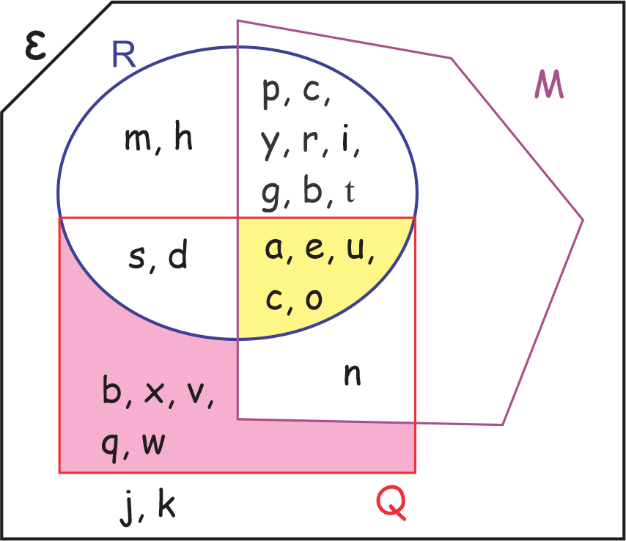
\includegraphics[width=0.65\textwidth]{figures/example1-1.png}
\end{center}

\begin{enumerate}
  \item List the elements in $R$, $M$, $Q$ and $\varepsilon$.
  \item Show that $R' \cap M' = (R \cup M)'$.
  \item Show that $(R \cap M \cap Q)' = R' \cup M' \cup Q'$.
\end{enumerate}
\medskip\noindent\textbf{Solution}
\begin{enumerate}
  \item
  \begin{align*}
    R &= \{s, u, b, d, e, r, m, a, t, o, g, l, y, p, h, i, c\}, \\
    M &= \{u, n, c, o, p, y, r, i, g, h, t, a, b, l, e\} \text{ and} \\
    Q &= \{a, e, u, c, o, n, x, q, v, w\} \text{ are subsets of} \\
    \varepsilon &= \{s, u, b, d, e, r, m, a, t, o, g, l, y, p, h, i, c, n, x, q, v, w, j, k\}.
  \end{align*}
  \item $R' \cap M' = (R \cup M)'$

  Let us first solve for $R' \cap M'$:
  \[
    \{b, x, v, n, q, w, j, k\} \cap \{m, h, s, d, b, x, v, q, w, j, k\}
  \]
  \[
    R' \cap M' = \{b, x, v, q, w, j, k\} \quad \ldots\ldots (1)
  \]
  Next, let us solve for $(R \cup M)'$:
  \[
    (R \cup M)' = \{s, u, b, d, e, r, m, a, t, o, g, l, y, p, h, i, c, n\}'
  \]
  \[
    (R \cup M)' = \{b, x, v, q, w, j, k\} \quad \ldots\ldots (2)
  \]
  Since equation (1) is equal to equation (2), it shows that $R' \cap M' = (R \cup M)'$.

  \textit{(Note: the original textbook's working reproduced above actually
  contains an arithmetic slip --- from the given $R$, $M$ and $\varepsilon$,
  the correct complements are $R' = \{j,k,n,q,v,w,x\}$ and
  $M' = \{d,j,k,m,q,s,v,w,x\}$ \emph{(no `b' or `h')}, giving
  $R'\cap M' = (R\cup M)' = \{j,k,q,v,w,x\}$ rather than the $\{b,x,v,q,w,j,k\}$
  shown above. The error appears on both sides of the equation, so it does
  not affect the conclusion that $R'\cap M'=(R\cup M)'$, but the specific set
  of elements shown is incorrect.)}

  \item Let's first solve for $(R \cap M \cap Q)'$:
  \[
    (R \cap M \cap Q)' = (a, e, u, c, o)'
  \]
  \[
    = \{s, b, d, r, m, t, g, l, y, p, h, i, n, x, q, v, w, j, k\} \quad \ldots\ldots (1)
  \]
  Next, let's find $R' \cup M' \cup Q'$:
  \begin{align*}
    R' \cup M' \cup Q' &= \{b, x, v, n, q, w, j, k\} \cup \{m, h, s, d, b, x, v, q, w, j, k\} \\
    &\quad \cup \{m, h, p, c, y, r, i, g, b, t, j, k\} \\
    &= \{s, b, d, r, m, t, g, l, y, p, h, i, n, x, q, v, w, j, k\} \quad \ldots\ldots (2)
  \end{align*}
  Since equation (1) is equal to equation (2), it shows $(R \cap M \cap Q)' = R' \cup M' \cup Q'$.

  \textit{(Note: this working carries the same erroneous $R'$ and $M'$ from
  part 2, plus a similarly erroneous
  $Q' = \{b,c,g,h,i,j,k,m,p,r,t,y\}$ instead of the correct
  $Q' = \{b,d,g,h,i,j,k,l,m,p,r,s,t,y\}$ \emph{(no `c'; includes `d', `l', `s')}.
  Taking the union of the textbook's own three (erroneous) complements gives
  $\{b,c,d,g,h,i,j,k,m,n,p,q,r,s,t,v,w,x,y\}$ --- note the `c' --- not the
  $\{s,b,d,r,m,t,g,l,y,p,h,i,n,x,q,v,w,j,k\}$ (with an `l' instead of a `c')
  printed above, so the final line does not even follow from the textbook's
  own stated $R'$, $M'$, $Q'$. The correct result, computed directly from
  $R\cap M\cap Q=\{a,c,e,o,u\}$, is
  $(R\cap M\cap Q)' = \varepsilon\setminus\{a,c,e,o,u\}
  = \{b,d,g,h,i,j,k,l,m,n,p,q,r,s,t,v,w,x,y\}$, which does agree with
  $R'\cup M'\cup Q'$ once the correct complements from the note above are
  used instead. As before, the identity itself still holds; only the
  specific elements printed in the textbook's arithmetic are unreliable.)}
\end{enumerate}
\end{example}
